\documentclass[10pt,twocolumn,letterpaper]{article}

\usepackage{times}
\usepackage{epsfig}
\usepackage{graphicx}
\usepackage{amsmath}
\usepackage{amssymb}
\usepackage{float}
\usepackage{mathtools}
\usepackage[noend]{algorithmic}
% \usepackage{algorithm,caption}
\usepackage{amsmath}
\usepackage{algorithm2e}
\DeclareMathOperator*{\argmin}{arg\,min}

% Include other packages here, before hyperref.

% If you comment hyperref and then uncomment it, you should delete
% egpaper.aux before re-running latex.  (Or just hit 'q' on the first latex
% run, let it finish, and you should be clear).
\usepackage[breaklinks=true,bookmarks=false]{hyperref}


\def\cvprPaperID{****} % *** Enter the CVPR Paper ID here
\def\httilde{\mbox{\tt\raisebox{-.5ex}{\symbol{126}}}}

% Pages are numbered in submission mode, and unnumbered in camera-ready
%\ifcvprfinal\pagestyle{empty}\fi
\setcounter{page}{1}
\date{October 26, 2017}
\begin{document}

%%%%%%%%% TITLE
\title{{Project Proposal CS221: Reinforcement Learning: Autonomous Race Car}}

\author{Olivier Pham\\
Stanford University\\
Management Science and Engineering\\
 {mdopham@stanford.edu}
% For a paper whose authors are all at the same institution,
% omit the following lines up until the university
% Additional authors and addresses can be added with ``\and'',
% just like the second author.
% To save space, use either the email address or home page, not both
\and
Stephanie Sanchez\\
Stanford University\\
Computational and Mathematical Engineering\\
{ ssanche2@stanford.edu}
\and
Vishal Subbiah\\
Stanford University\\
Computational and Mathematical Engineering\\
{svishal@stanford.edu}
}
\maketitle
%\thispagestyle{empty}

%%%%%%%%% ABSTRACT
%\begin{abstract}
  

%\end{abstract}

%%%%%%%%% BODY TEXT
\section*{Presentation of the project}

%-------------------------------------------------------------------------

Autonomous vehicles for real world environment have been a long term ambition and in recent years endeavors towards this objective have shown very promising results. But what about autonomous driving for video games? If we can simulate autonomus driving in a game, it may give further insight to applying it in the real world. We propose to implement Reinforcement Learning (RL) to train an agent in the Open AI gym Atari game, Enduro-v0. The original goal of the game was to attain the maximum points but we decided to see if our agent could reach first place among 200 other cars. The goal is for the agent to learn from its environment and actions, the intention of the game and develop an optimal policy to win.
\begin{figure}[h]
\centering
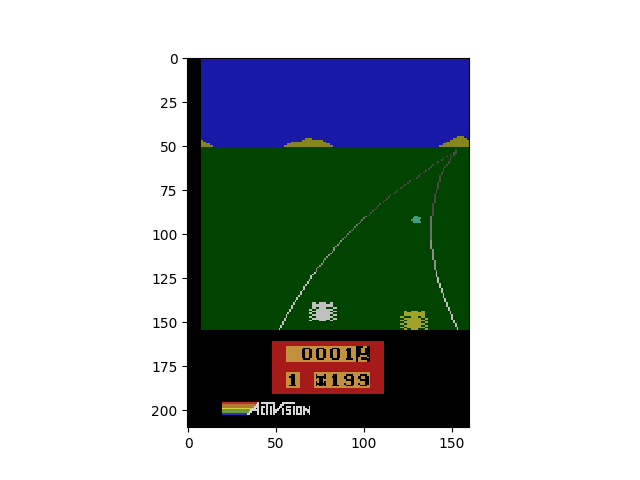
\includegraphics[width=0.8\linewidth]{img81.png}
\caption{Screenshot from the game}
\end{figure}
%-------------------------------------------------------------------------

\section*{Inputs and Outputs}

We will be using the OpenAI Gym environment for this project. \\
This environment provides us with pixels, rewards and a boolean indicating if the episode has ended (which happens after 13 300 frames). The observation space is a 210*160 pixels 8-bit RGB image of the screen which is represented by an array of size (210, 160, 3).\\
There are 9 possible actions which are:
\begin{itemize}
\itemsep-0.2em 
\item No Operation
\item Accelerate
\item Move Right
\item Move Left
\item Brake
\item Brake Right
\item Brake Left
\item Accelerate Right
\item Accelerate Left
\end{itemize}

For every state and action, the default reward is defined the following way: \[ \text{Reward(s,a,s')} = \begin{cases}1 & \text{when overtaking a car}\\-1 & \text{when crashing into another car} \\0 & \text{otherwise}\end{cases}\]


However, as the goal of the project is to learn a policy for reaching the first position as quickly as possible, we will use the following reward:
\[\text{Reward(s,a,s')} = - \text{Position in the race at the state s'}\]
We will extract the position in the race from the RGB image using a machine learning or rule based digits classifier.



%-------------------------------------------------------------------------
\section*{Metrics}

Our first goal will be to reach the first position before the end of the game while reducing the number of cars hit. To measure our success we will assess our position at the end of the race, since we bounce backwards if we hit another car.\\

We could also explore delaying the reward to see how well the agent behaves with limited feedback. Another possible exploration is to introduce stochasticity by assigning a certain probability to the action chosen.
\\

If we manage to reach the goal and its variations, our next objective will be to reach the first position as quickly as possible. Therefore, the metric we will measure and try to minimize the number of frames required to reach the first position.



%The agent's performance will be evaluated against human performance. Aspects for assessment include: time to complete the race, racing position upon race completion, and objects hit during the race. 


%-------------------------------------------------------------------------

\section*{Baseline and Oracle}

The Oracle for this project is to reach the first position at the end of the episode, hence its success metric is 1.\\

Our baseline is a simple approach which is to accelerate at every time step without trying to avoid other cars. After 10 games, we get an average final position of 184/200.

%-------------------------------------------------------------------------
\section*{Methods Used To Solve The Problem}

Previous work for RL and car racing used pixel values and rewards from the gym environment to learn optimal policy \cite{Car-Racing}. Other work that includes learning Atari games involves raw pixels as inputs and outputs a function that estimates future rewards that is generated by coupling of a Convolutional Neural Network (CNN) with a form of Q-Learning \cite{DeepMind}. A last take on playing Atari games defines a constant model and hyperparameter settings for the RL algorithms with a classical input features from Atari environment into the algorithms \cite{HyperParam}. \\

Some of the challenges we will face is the large state space since its a continuous game (and not turn based) and we are using the raw pixels.

\begin{thebibliography}{9}
\bibitem{Car-Racing} 
M. A. Farhan Khan, Oguz H. Elibol
\textit{Car Racing using Reinforcement Learning}. 

 
\bibitem{DeepMind} 
Volodymyr Mnih, Koray Kavukcuoglu, David Silver, Alex Graves, Ioannis Antonoglou,
Daan Wierstra, Martin Riedmiller
\textit{Playing Atari with Deep Reinforcement Learning}. 


\bibitem{HyperParam} 
David Hershey, Rush Moody, Blake Wulfe
\textit{Learning to Play Atari Games}. 

\end{thebibliography}
\end{document}
